\subsection{Pjproject e i driver audio: OpenSL-ES}\label{subsubsec:OnlyAudioOpenSles}
\textit{Per la descrizione della particolare implementazione delle API OpenSL ES
da parte di Android detta \texttt{wilhelm}, si veda la Sottosezione \vref{subsec:mischeWilhelm}.}
\bigskip

OpenSL-ES è, come dicono gli stessi sviluppatori \parencite{man:opensles}, un'API
realizzata per sistemi \textit{embedded} e \textit{mobili} con il supporto
per la multimedialità, che fornisce un'interfaccia audio indipendente dal
device ed il più possibile \textit{cross-platform}. È inoltre sviluppata tenendo
conto delle ristrette risorse disponibili di questi dispositivi ed utilizzando
API \textit{object-oriented}, che fanno assomigliare il codice C a quello di linguaggi
quale il C++, con un approccio simile a quello già descritto in Pjproject.

Posso mostrare brevemente quale sia l'interfaccia utilizzata per interagire con
gli oggetti descrivendo l'interfaccia base per tutti gli oggetti, ovvero quella
fornita da \texttt{\small SLObjectItf}.


Come possiamo notare dalla Figura \subref{subfig:statesldiagram} \vref{fig:Opensles},
all'atto della creazione dell'oggetto questo è \textit{unrealized}: ciò vuol dire che le sue risorse 
non sono state ancora allocate e non è inoltre possibile 
utilizzare i metodi esposti dalle sue interfacce. Per effettuare la transizione
allo stato \textit{realized}, è necessario invocare l'omonimo metodo (\texttt{\small Realize})
sull'oggetto in questione.

\begin{figure}[thp]
\centering
\subfloat[][\textit{Posizione della libreria OpenSL ES all'interno di un sistema operativo: l'implementazione Wilhelm è del secondo tipo, in quanto interagisce direttamente con le librerie di sistema. \url{http://www.khronos.org/opensles/}}]{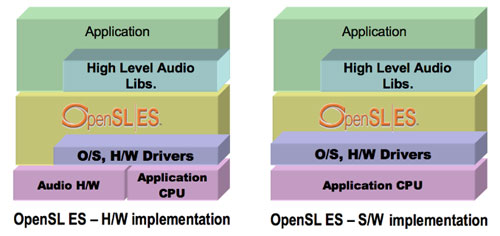
\includegraphics[scale=0.9]{img/libraries/opensles_sw_hw1.png}}\\
\subfloat[][\textit{Diagramma degli oggetti mostrante l'interazione tra oggetti nei vari livelli del codice. \parencite{man:opensles}}]{\label{subfig:statesldiagram}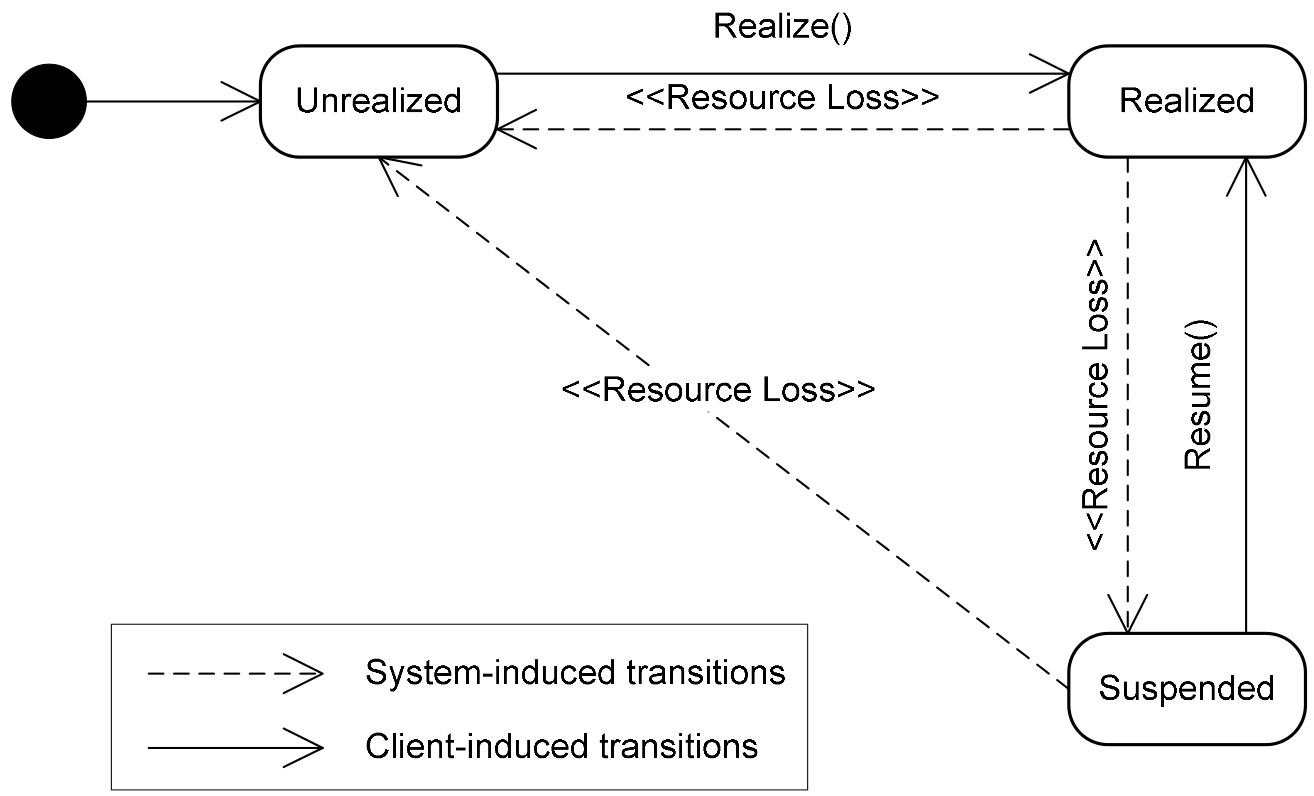
\includegraphics[scale=0.25]{img/libraries/slobject.png}}\\
\caption{OpenSL ES.}
\label{fig:Opensles}
\end{figure}

Tuttavia l'interazione con i suddetti oggetti è possibile unicamente previa
istanziazione dell'\textit{Engine Object}, tramite la funzione globale \texttt{\small slCreateObject()},
la quale fornirà appunto un'istanza del sistema, per mezzo della quale è possibile 
ottenere nuove istanze di oggetti, le cui interfacce sono già descritte all'interno
del sistema. Un utilizzo dell'implementazione di tale API è fornita all'interno
del file \texttt{\small opensl\_dev.c} della libreria Pjproject nel branch Android,
che ho quindi deciso di adottare in quanto questa versione aveva nel frattempo 
implementato i device per la gestione dell'audio.

In prima analisi, noto come \texttt{\small CreateAudioInterface} sia 
	un puntatore a funzione della \texttt{\small struct SLEngineItf\_} definita 
	all'interno di \textit{OpenSLES.h}, che è a sua volta il tipo della variabile 
	\texttt{\small engineEngine} all'interno della definizione del driver audio 
	nel file  \texttt{\small opensl\_dev.c}. In pratica posso osservare come
	l'implementazione di \texttt{\small src/itf/IEngine.c} associ a tale 
puntatore la funzione \texttt{\small IEngine\_CreateAudioPlayer}.

\subsubsection{Patch per il device audio (\texttt{android\_sles\_dev.c}) e branch Android}
Utilizzando la versione \textit{trunk} di \texttt{\small pjsip} e crosscompilandola con 
la patch trovata all'interno della mailing-list di Android, all'atto dell'instaurazione
della chiamata, riscontro il seguente errore:
\begin{bash}
23:10:04.169   pjsua_call.c !Making call with acc #1 to sip:192.168.0.9
23:10:04.169    pjsua_aud.c  .Set sound device: capture=-1, playback=-2
23:10:04.169    pjsua_aud.c  ..Error retrieving default audio device parameters: Unable to find default audio device (PJMEDIA_EAUD_NODEFDEV) [status=420006]
\end{bash}
A causa di questo problema, ho optato per l'utilizzo della versione \textit{branch} 
per Android, anche perché questa versione è stata corredata per i codec wav, che 
sembrano mancanti nella versione \textit{trunk}, ed è  da 
ritenersi maggiormente completa. Di fatti a quanto pare il patch indicato non
sembra effettuare correttamente l'ottenimento dei parametri di default, e nemmeno
è in grado di ottenere il device audio predefinito. 

